% \begin{figure}[t]
% \centering

% \subfloat[
%     \textbf{CIFAR-100 50+50.}
%     \label{fig:partial_zip_cifar100}
% ]{
% \centering
% \begin{minipage}{0.49\linewidth}{
% \begin{center}
%     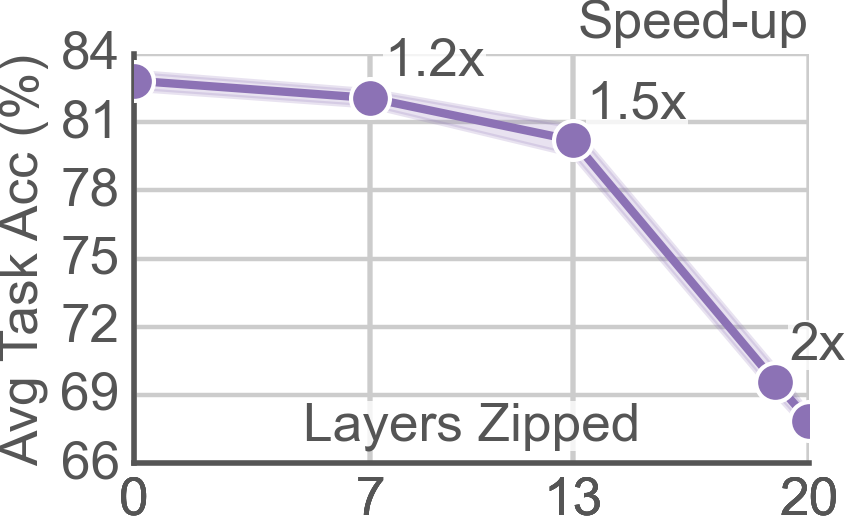
\includegraphics[width=\linewidth]{figures/imgs/partial_zip_CIFAR_50_50.png}
% \end{center}
% }\end{minipage}
% }
% \subfloat[
%     \textbf{ImageNet-1k 200+200.}
%     \label{fig:partial_zip_imagenet}
% ]{
% \centering
% \begin{minipage}{0.49\linewidth}{
% \begin{center}
%     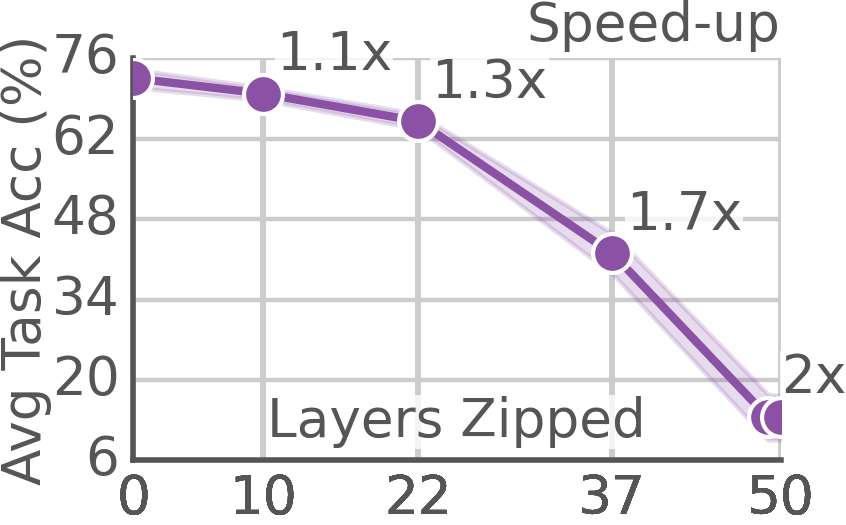
\includegraphics[width=\linewidth]{figures/imgs/partial_zip_imnet_200_200.png}
% \end{center}
% }\end{minipage}
% }

% \caption{
% {\bf Varying Partial Zip.} 
% By leaving some layers unzipped (Sec.~\ref{sec:partial_zip}), we can recover a significant amount of performance while still merging most of the model. 
% }
% \label{fig:varying_partial_zip}
% \end{figure}

% \begin{wrapfigure}{r}{0.48\linewidth}
% \vspace{-10pt}
% \centering
% \resizebox{\linewidth}{!}{
%     \tablestyle{5pt}{1.1}
%     {
%     \tablestyle{5pt}{1.1}
%     \begin{tabular}{x{40}x{40}x{40}}
%         \multicolumn{3}{c}{Average Stage Correlations}\\
%         Layer \sfrac{7}{20} & Layer \sfrac{13}{20} & Layer \sfrac{19}{20}\\
%     \shline
%     {0.50\conf{0.01}} & {0.37\conf{0.00}} & {0.27\conf{0.00}} \\
%     \hline
% \end{tabular}
%     }
% }
% \captionof{table}{\textbf{CIFAR-100 (50+50) Zipping Correlations.} We show the average correlations between two ResNet-20 ($8\times$) models at each partial zipping stage. Correlations consistently decrease at each successive stage, indicating that the layers of the two models increasingly diverge. 
% }
% \label{tab:partialzip_corrs}
% % \end{table}
% \vspace{-20pt}
% \end{wrapfigure}


\begin{wrapfigure}{r}{0.48\linewidth}
\vspace{-15pt}
\begin{minipage}[l]{\linewidth}{
\captionsetup{justification=centering}
\subfloat[
    \textbf{CIFAR-100 \\ \ \ \ \ (50+50)}
    \label{fig:partial_zip_cifar100}
]{
\centering
\begin{minipage}{0.48\linewidth}{
\begin{center}
    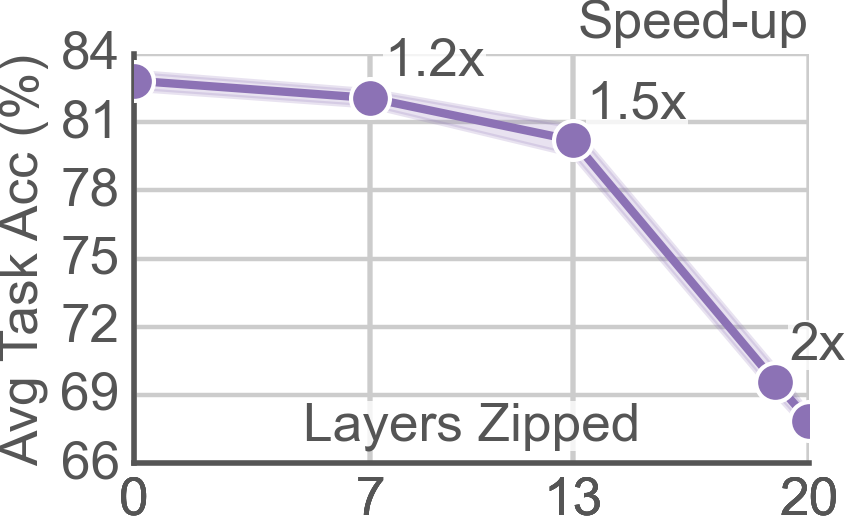
\includegraphics[width=\linewidth]{figures/imgs/partial_zip_CIFAR_50_50.png}
\end{center}
}\end{minipage}
}
\subfloat[
    \textbf{ImageNet-1k \\ \ \ \  (200+200)}
    \label{fig:partial_zip_imagenet}
]{
\centering
\begin{minipage}{0.48\linewidth}{
\begin{center}
    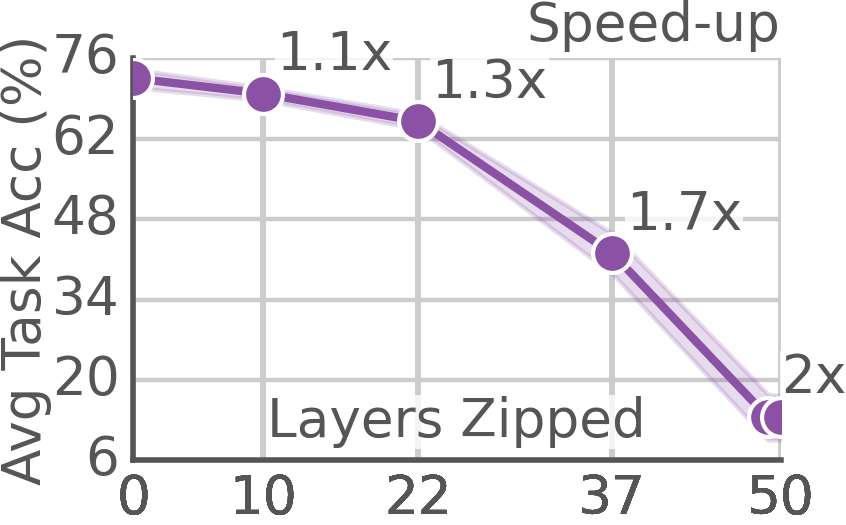
\includegraphics[width=\linewidth]{figures/imgs/partial_zip_imnet_200_200.png}
\end{center}
}\end{minipage}
}
\captionsetup{justification=justified}
        \caption{{\bf Varying Partial Zip.} By leaving some layers unzipped (Sec.~\ref{sec:partial_zip}), we can recover a significant amount of performance while still merging most of the model. }
\label{fig:varying_partial_zip}
}\end{minipage}
\begin{minipage}[l]{\linewidth}{
\vspace{5pt}
\centering
\resizebox{\linewidth}{!}{
    \tablestyle{5pt}{1.1}
    {
    \tablestyle{5pt}{1.1}
    \begin{tabular}{x{40}x{40}x{40}}
        \multicolumn{3}{c}{Average Stage Correlations}\\
        Layer \sfrac{7}{20} & Layer \sfrac{13}{20} & Layer \sfrac{19}{20}\\
    \shline
    {0.50\conf{0.01}} & {0.37\conf{0.00}} & {0.27\conf{0.00}} \\
    \hline
\end{tabular}
    }
}
\captionof{table}{\textbf{CIFAR-100 (50+50) Zipping Correlations.} We show the average correlations between two ResNet-20 ($8\times$ width) models at each partial zipping stage. Correlations consistently decrease at each successive stage, indicating that the layers of the two models increasingly diverge. 
}
\label{tab:partialzip_corrs}
% \end{table}
% \vspace{10pt}
}\end{minipage}
\begin{minipage}[l]{\linewidth}{
\captionsetup{justification=centering}
\vspace{1em}
\subfloat[
    \textbf{CIFAR-100 \\ \ \ \ \ (50+50)}
    \label{fig:data_use_cifar100}
]{
\centering
\begin{minipage}{0.48\linewidth}{
\begin{center}
    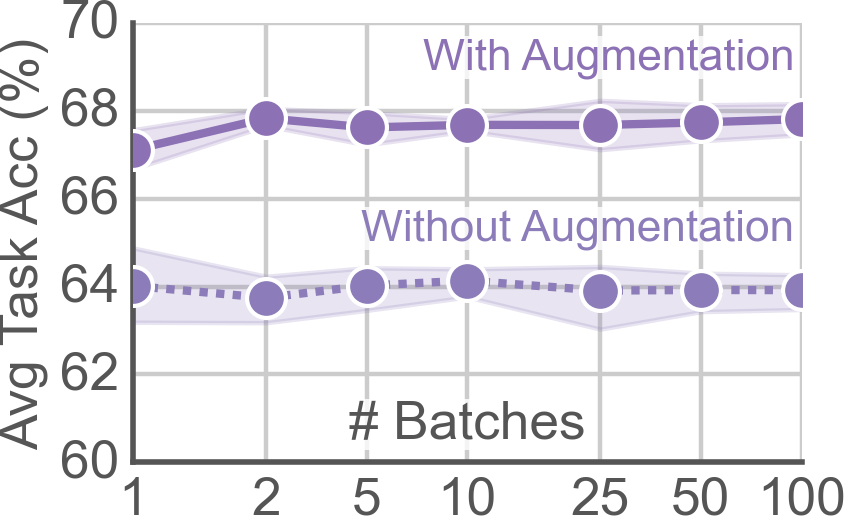
\includegraphics[width=\linewidth]{figures/imgs/cifar100_data.png}
\end{center}
}\end{minipage}
}
\subfloat[
    \textbf{ImageNet-1k \\ \ \ \  (200+200)}
    \label{fig:data_use_imagenet}
]{
\centering
\begin{minipage}{0.48\linewidth}{
\begin{center}
    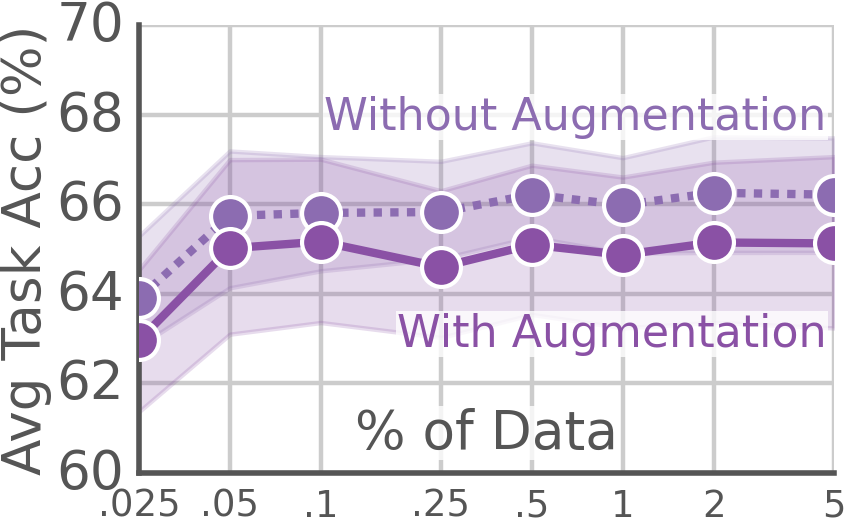
\includegraphics[width=\linewidth]{figures/imgs/imnet200_data.png}
\end{center}
}\end{minipage}
}
\captionsetup{justification=justified}
\caption{
{\bf Data Usage.} 
How much data do we need to use to compute activations? 
We find that only a few hundred images are needed to obtain the best performance.
Data augmentation is not always useful.
% Here we ablate the amount of data used for our CIFAR-100 (50+50) ResNet-20 ($8\times$ width) and ImageNet (200+200) Resnet-50 (\sfrac{22}{50} layers) experiments. 
% The batch size used is 500 for CIFAR and 16 for ImageNet. 
% In both cases, we only need a few hundred images to obtain the best results. 
% On the other hand, data augmentation is necessary for CIFAR but hurts for ImageNet. Our default for all experiments uses data augmentation and the full set for CIFAR (100 batches) and 1\% of the data for ImageNet. 
}
\label{fig:data_usage}
}\end{minipage}
% \vspace{-60pt}
\end{wrapfigure}

% \begin{wrapfigure}{l}{0.52\linewidth}
% % \vspace{-260pt}
% \begin{minipage}[l]{\linewidth}{
% \subfloat[
%     \textbf{CIFAR-100 (50+50).}
%     \label{fig:data_use_cifar100}
% ]{
% \centering
% \begin{minipage}{0.48\linewidth}{
% \begin{center}
%     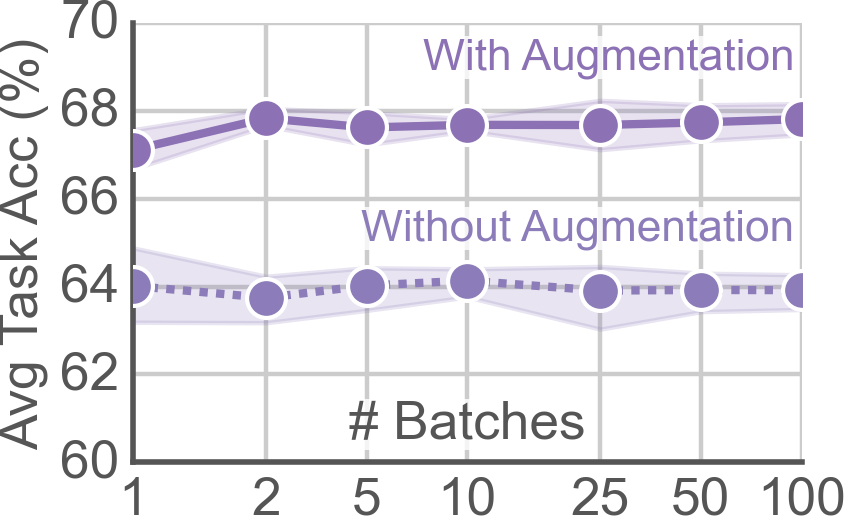
\includegraphics[width=\linewidth]{figures/imgs/cifar100_data.png}
% \end{center}
% }\end{minipage}
% }
% \subfloat[
%     \textbf{ImageNet-1k (200+200).}
%     \label{fig:data_use_imagenet}
% ]{
% \centering
% \begin{minipage}{0.48\linewidth}{
% \begin{center}
%     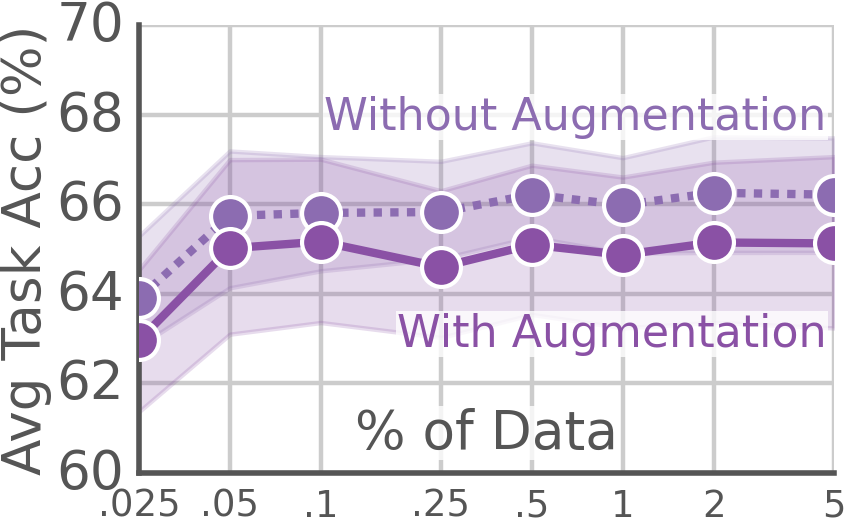
\includegraphics[width=\linewidth]{figures/imgs/imnet200_data.png}
% \end{center}
% }\end{minipage}
% }
%         \caption{
%         {\bf Data Usage.} How much data do we need to use to compute activations? Here we ablate the amount of data used for our CIFAR-100 (50+50) ResNet-20 ($8\times$ width) and ImageNet (200+200) Resnet-50 (\sfrac{22}{50} layers) experiments. The batch size used is 500 for CIFAR and 16 for ImageNet. In both cases, we only need a few hundred images to obtain the best results. On the other hand, data augmentation is necessary for CIFAR but hurts for ImageNet. Our default for all experiments uses data augmentation and the full set for CIFAR (100 batches) and 1\% of the data for ImageNet. 
%         }
% \label{fig:data_usage}
% }\end{minipage}
% \end{wrapfigure}


% \caption{{\bf Data Usage.} How much data do we need to use to compute activations? Here we ablate the amount of data used for our CIFAR-100 (50+50) ResNet-20 ($8\times$ width) and ImageNet (200+200) Resnet-50 (\sfrac{22}{50} layers) experiments. The batch size used is 500 for CIFAR and 16 for ImageNet. In both cases, we only need a few hundred images to obtain the best results. On the other hand, data augmentation is necessary for CIFAR but hurts for ImageNet. Our default for all experiments uses data augmentation and the full set for CIFAR (100 batches) and 1\% of the data for ImageNet. }
% \label{fig:data_usage}
% \end{figure}


% \begin{figure}
%     \begin{minipage}[t]{0.50\linewidth}
%         \centering
%         \subfloat[
%             \textbf{CIFAR-100 (50+50).}
%             \label{fig:partial_zip_cifar100}
%         ]{
%             \centering
%             \begin{minipage}{0.40\linewidth}{
%                 \centering
%                 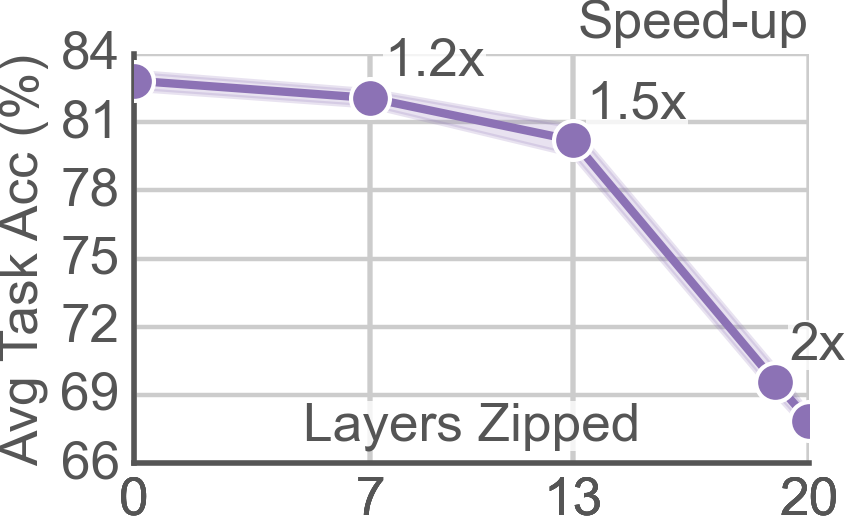
\includegraphics[width=\linewidth]{figures/imgs/partial_zip_CIFAR_50_50.png}
%             }\end{minipage}
%         }
%         \subfloat[
%             \textbf{ImageNet-1k (200+200).}
%             \label{fig:partial_zip_imagenet}
%         ]{
%             \centering
%             \begin{minipage}{0.40\linewidth}{
%                 \centering
%                 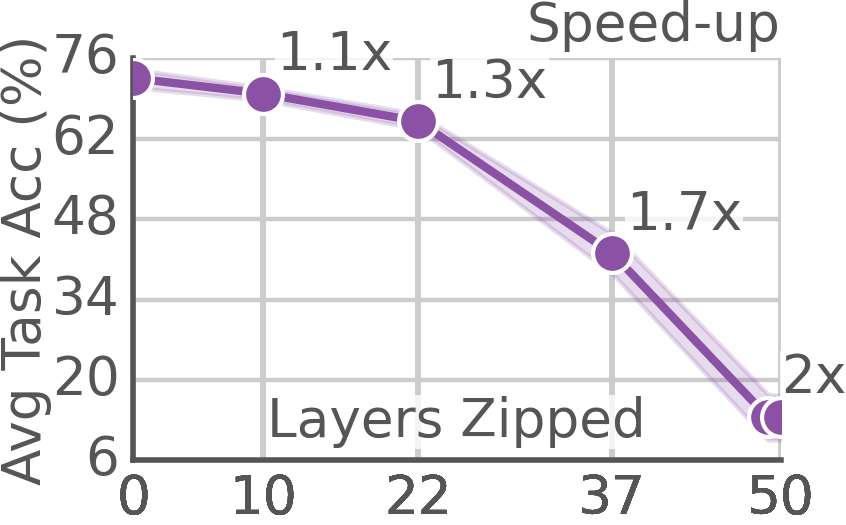
\includegraphics[width=\linewidth]{figures/imgs/partial_zip_imnet_200_200.png}
%             }\end{minipage}
%         }
%         \caption{{\bf Varying Partial Zip.} 
%             By leaving some layers unzipped (Sec.~\ref{sec:partial_zip}), we can recover a significant amount of performance while still merging most of the model.  }
%         \label{fig:varying_partial_zip}
%         % \vspace{-80pt}
%     \end{minipage}
%     \hspace{1pt}
%     % \vspace{1em} % Add vertical space between the images
%     \begin{minipage}[t]{0.48\linewidth}
%         \centering
%         \subfloat[
%             \textbf{CIFAR-100 (50+50).}
%             \label{fig:data_use_cifar100}
%         ]{
%             \centering
%             \begin{minipage}{0.48\linewidth}{
%                 \centering
%                 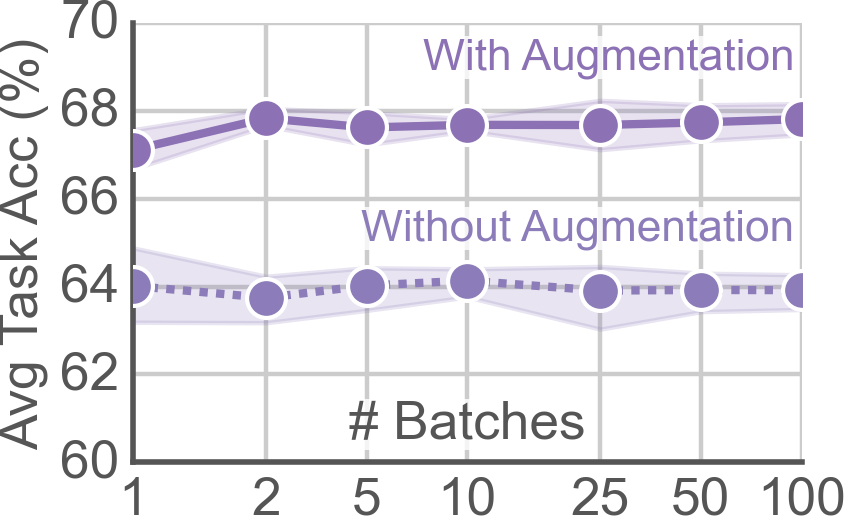
\includegraphics[width=\linewidth]{figures/imgs/cifar100_data.png}
%             }\end{minipage}
%         }
%         \subfloat[
%             \textbf{ImageNet-1k (200+200).}
%             \label{fig:data_use_imagenet}
%         ]{
%             \centering
%             \begin{minipage}{0.48\linewidth}{
%                 \centering
%                 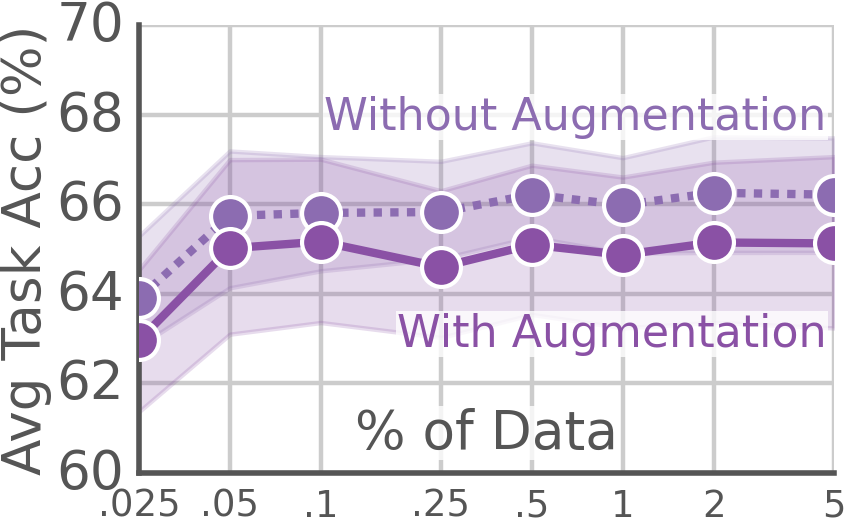
\includegraphics[width=\linewidth]{figures/imgs/imnet200_data.png}
%             }\end{minipage}
%         }
%         \caption{
%         {\bf Data Usage.} How much data do we need to use to compute activations? Here we ablate the amount of data used for our CIFAR-100 (50+50) ResNet-20 ($8\times$ width) and ImageNet (200+200) Resnet-50 (\sfrac{22}{50} layers) experiments. The batch size used is 500 for CIFAR and 16 for ImageNet. In both cases, we only need a few hundred images to obtain the best results. On the other hand, data augmentation is necessary for CIFAR but hurts for ImageNet. Our default for all experiments uses data augmentation and the full set for CIFAR (100 batches) and 1\% of the data for ImageNet. 
%         }
%         \label{fig:data_usage}
%         % \vspace{10pt}
%     \end{minipage}
%     % \caption{Overall caption for the three images}
%     \vspace{-20pt}
% \end{figure}